\chapter{Cahier des charges}
\label{chapter1}

%Introduction
%Spécifications techniques
%	en résumé
%Organisation > répartition, trello, github, slack
%étude de solutions techniques

%part Cahier des charges
%part Structure 3D
%part Hardware
%part Middleware
%part Software
%part Conclusion



\section{Introduction}

Le but de ce projet est de réaliser un télescope électronique. C'est-à-dire un télescope doté d'une caméra et dont les mouvements sont pilotables via une interface homme-machine.

\vspace{1cm}

Ce projet se base sur un projet existant~: un télescope de type Newton conçu pour être imprimable à l'imprimante 3D.

Lien du projet~: \url{https://blog.dagoma.fr/telescope-imprime-en-3d/}

\begin{figure}[H]
	\centering
    \includegraphics[width=0.9\linewidth]{\figures/telescope-imprime-3D-5.jpg}
    \decoRule
    \caption[
    Photo du télescope imprimé]{
    Photo du télescope imprimé}
    \label{fig:Photo du télescope imprimé}
	\end{figure}



\section{Spécifications techniques}

Certaines fonctionnalités devront impérativement être implémentées pour que le télescope soit validé. D'autres sont envisagées et seront implémentées dans la mesure du possible avant l'évaluation de ce projet. Certaines le seront éventuellement passé cette date, d'autres ne le seront peut être jamais.

De plus nous nous imposons dès le départ l'utilisations de certains matériels.

\subsection{Fonctionnalités obligatoires}

Le télescope devra être capable d'effectuer des mouvements d'azimut à 360\textdegree et des mouvements d'élévation dont l'amplitude dépend de la structure du télescope utilisé comme point de départ.

\vspace{1cm}

Il disposera d'une caméra permettant de prendre des clichés.

\vspace{1cm}

Concernant l'interface homme-machine, il disposera d'une interface réseau rudimentaire ainsi que d'un écran tactile. Il sera donc doté d'un logiciel de pilotage.

\subsection{Fonctionnalités envisagées}

Le pilotage du télescope via une interface web est sérieusement envisagé.

\vspace{1cm}

D'autres fonctionnalités logicielles plus évoluées telles qu'un dispositif d'amélioration de la qualité des images ou un logiciel de traçage / reconnaissance d'astre seront étudiées.

Idéalement ces solutions seront embarquées dans le télescope, toutefois la possibilité de les déporter vers un serveur distant d'une plus grande puissance de calcul n'est pas exclue.

Ces fonctionnalités étant estimées d'une complexité importante, il est probable que leur développement demande beaucoup de temps et qu'elles ne soient pas terminées à la fin du projet.

\vspace{1cm}

L'ajout d'une batterie permettant l'autonomie du télescope est également envisagé mais n'est pas vu comme une priorité.

\subsection{Matériel}

Nous avons choisi d'utiliser comme élément central un SoC (System on Chip) industrialisable, ce qui exclut l'usage des cartes Raspberry Pi par exemple. Nous avons retenu la carte PICO-PI-IMX7D de NXP.

Cette carte est composé d'un module PICO-IMX7D équipé d'un processeur IMX7D et d'une carte d'interface format Raspberry Pi.

\begin{figure}[H]
	\centering
    \includegraphics[height=0.3\linewidth]{\figures/PICO-IMX_System-on-Module.png}
	\hspace{1cm}
    \includegraphics[height=0.3\linewidth]{\figures/PICO-PI.png}
    \decoRule
    \caption[
    Module PICO-IMX7D à droite et carte PICO-PI à gauche]{
    Module PICO-IMX7D à droite et carte PICO-PI à gauche}
    \label{fig:Module PICO-IMX7D à droite et carte PICO-PI à gauche}
	\end{figure}
 
\vspace{1cm}

La caméra et l'écran choisis font partie du "Starter kit" commercialisé avec la carte et sont de références respectives Omnivision ov5645 et Chimei Innolux EJ050NA-01G.

La caméra pourra éventuellement être remplacée par une caméra plus performante si le besoin s'en fait ressentir.

\subsection{Résumé des exigences}

\begin{figure}[H]
	\centering
    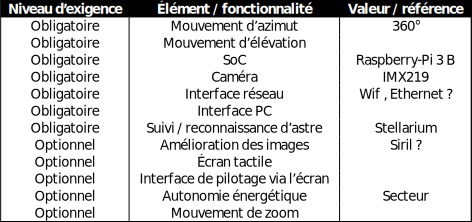
\includegraphics[width=0.7\linewidth]{\figures/tab_exigences.pdf}
    \decoRule
    \caption[
    Tableau récapitulatif des exigences du projet]{
    Tableau récapitulatif des exigences du projet}
    \label{fig:Tableau récapitulatif des exigences du projet}
	\end{figure}



\section{Organisation}

%outils
%répartition du travail

En tant que groupe de quatre personne, nous avons choisi de travailler en appliquant les méthodes agiles. Ainsi la répartition du travail au sein du groupe se fera de façon dynamique en fonction des aptitudes de chacun et de la charge de travail nécessaire pour terminer une tache donnée en un temps imparti.

\vspace{1cm}

Nous avons sélectionné quelques outils pour travailler de façon optimale~:
\begin{itemize}[label=$\bullet$]
	\item {\href{https://slack.com}{Slack}} comme moyen de communication.
	\item {\href{https://trello.com}{Trello}} comme outil de gestion de projet.
	\item {\href{https://github.com}{Github}} comme hébergeur de code source.
	\begin{itemize}
		\item Dépôt dédié à la layer Yocto du système d'exploitation de la PICO-PI~:\\\url{https://github.com/thomaslepoix/meta-autoscope}
		\item Dépôt dédié aux autres éléments du projet~:\\\url{https://github.com/thibaudledo/Autoscope}
		\end{itemize}
	\end{itemize}

\vspace{1cm}

À l'issue d'une étude technique préliminaire, nous avons dressé un schéma fonctionnel provisoire du système.

\begin{figure}[H]
	\centering
    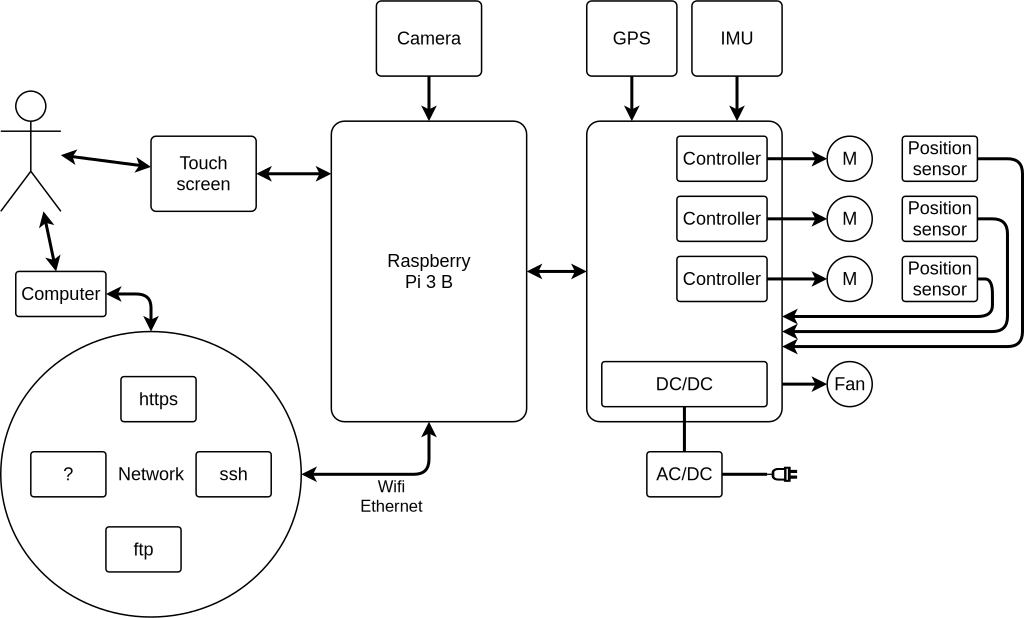
\includegraphics[width=0.8\linewidth]{\figures/sch_functionnal.pdf}
    \decoRule
    \caption[
    Schéma fonctionnel provisoire du système électronique du télescope]{
    Schéma fonctionnel provisoire du système électronique\\du télescope}
    \label{fig:Schéma fonctionnel provisoire du système électronique du télescope}
	\end{figure}

\vspace{1cm}

Nous avons donc pu trier et organiser les différentes tâches à accomplir et en prioriser certaines représentées en orange sur le diagramme ci-dessous. Les tâches encadrées de gras sont celles jugées les plus critiques pour l'accomplissement du projet.

\begin{figure}[H]
	\centering
    \includegraphics[width=1\linewidth]{\figures/sch_gantt_6.pdf}
    \decoRule
    \caption[
    Diagramme de l'organisation temporelle du travail sur le projet]{
    Diagramme de l'organisation temporelle du travail sur le projet}
    \label{fig:Diagramme de l'organisation temporelle du travail sur le projet}
	\end{figure}

